%%% Для сборки выполнить 2 раза команду: pdflatex <имя файла>

\documentclass[a4paper,12pt]{article}
\usepackage{setspace} 
\usepackage{ucs}
\usepackage[utf8x]{inputenc}
\usepackage[russian]{babel}
%\usepackage{cmlgc}
\usepackage{graphicx}
\usepackage{listings}
\usepackage{xcolor}
\usepackage[labelformat=simple]{subcaption}
%\usepackage{courier}

\makeatletter
\renewcommand\@biblabel[1]{#1.}
\makeatother

\newcommand{\myrule}[1]{\rule{#1}{0.4pt}}
\newcommand{\sign}[2][~]{{\small\myrule{#2}\\[-0.7em]\makebox[#2]{\it #1}}}

% Поля
\usepackage[top=20mm, left=30mm, right=10mm, bottom=20mm, nohead]{geometry}
\usepackage{indentfirst}

% Межстрочный интервал
\renewcommand{\baselinestretch}{1.50}


\begin{document}

%%%%%%%%%%%%%%%%%%%%%%%%%%%%%%%
%%%                         %%%
%%% Начало титульного листа %%%

\thispagestyle{empty}

\begin{center}
	
	
	\renewcommand{\baselinestretch}{1}
	{\large
		{\sc Петрозаводский государственный университет\\
			Институт математики и информационных технологий\\
			Кафедра информатики и математического обеспечения}
		}
	Направление подготовки бакалавриата \\ 09.03.04 - Программная инженерия	
\end{center}
 
\vfill

\begin{center}
{\normalsize Экзаменационная работа по дисциплине "Проектирование информационных систем"\\ С предметной областью } \\

\medskip

%%% Название работы %%%
{\Large \sc  Зубная поликлиника \\
	 
}
 
\end{center}

\medskip

\begin{flushright}
\parbox{11cm}{%
\renewcommand{\baselinestretch}{1.2}
\normalsize
Выполнил:\\
%%% ФИО студента %%%
студент 3 курса группы 22307 В. А. Аверков
\begin{flushright}
\sign[подпись]{4cm}
\end{flushright}

студентка 3 курса группы 22307 Д. В. Горбунова
\begin{flushright}
	\sign[подпись]{4cm}
\end{flushright}

Место прохождения обучения: \\ { кафедра прикладной математики и кибернетики}\\

Период прохождения обучения: 02.09.19-27.12.19 \\
% Раскмментируйте строку с нужным Вам периодом прохождения.
%	\textcolor{red}{Для 4 к. бакалавриата и 6 к. магистратуры:} \\
% Период прохождения практики: \\ 02.09.19-15.12.19 \\
%	\textcolor{red}{Для остальных курсов:} \\
% Период прохождения практики: \\ 02.09.19-22.12.19 \\

% Если руководителей два - то раскомментровать строку про второго руководителя и применть "Руководители:"

Руководитель:\\
%%% степень, звание ФИО научного руководителя %%%
% Первый руководитель 
{Л. В. Щеголева, профессор} \\
\begin{flushright}
	\sign[подпись]{4cm}
\end{flushright}







Итоговая оценка
\begin{flushright}
	\sign[оценка]{4cm}
\end{flushright}
}
\end{flushright}
\vfill
\begin{center}
\large
Петрозаводск --- 2019
\end{center}

%%% Конец титульного листа  %%%
%%%                         %%%
%%%%%%%%%%%%%%%%%%%%%%%%%%%%%%%

%%%%%%%%%%%%%%%%%%%%%%%%%%%%%%%%
%%%                          %%%
%%% Содержание               %%%

\newpage

\tableofcontents

%%% Содержание              %%%
%%%                         %%%
%%%%%%%%%%%%%%%%%%%%%%%%%%%%%%%


%%%%%%%%%%%%%%%%%%%%%%%%%%%%%%%%
%%%                          %%%
%%% Введение                 %%%

%%% В введении Вы должны описать предметную область, с которой связана %%%
%%% Ваша работа, показать её актуальность, вкратце определить цель     %%%
%%% исследования/разработки					       %%%

\newpage
\section*{Введение}
\addcontentsline{toc}{section}{Введение}

\par Платная зубная клиника оказывает услуги по лечению зубов. Клиника обслуживает частных пациентов. Клиника заключает договора с организациями на обслуживание их сотрудников. Организация оплачивает лечение своих сотрудников в размере, не превышающем определенной суммы, остальную часть пациент оплачивает сам. Необходимо обеспечить информационную поддержку деятельности по учету пациентов, договоров и оплате выполненных услуг частных пациентов и организаций.


\newpage
\section{Бизнес требования и дерево функций}
\subsection{Бизнес требования}
Информационная система «Зубная поликлиника» обеспечивает возможности:

\begin{enumerate}

\item Упростить возможность отчетности о заключаемых договорах c организациями:
\begin{enumerate}
\item  Просматривать список заключенных договоров.

\item Редактировать список заключенных договоров.

\item Просматривать список рабочих для каждой организации.

\item  Редактировать список работников для каждой организации.
\end{enumerate}
\item Упростить процесс заключения договоров с организациями.
\begin{enumerate}
\item Составлять список сотрудников организации.

\item Фиксировать стоимость услуг, покрываемых организацией.
\end{enumerate}




\item Упростить возможность отчетности о клиентах от организаций и частных клиентах и оказываемых им услугах.
\begin{enumerate}
\item Просматривать список клиентов.

\item Просматривать список оказанных услуг для каждого клиента.

\item Редактировать список клиентов.

\item  Редактировать список оказанных услуг для каждого клиента.
\end{enumerate}
\item Упростить вычисления стоимости оказанных услуг для клиентов от организаций, учитывая часть, оплачиваемую фирмой и предоставление чека для частных клиентов и клиентов от организаций.
\begin{enumerate}
\item  Просмотр отчета о клиентах и услугах.

\item  Просмотр оплачиваемой стоимости.
\item  Редактирование оплачиваемой стоимости.

\item  Просмотр оставшейся стоимости.
\end{enumerate}
\item  Ввести систему аутентификации.
\begin{enumerate}
\item   Логин/пароль. (Один и более администраторов)
\end{enumerate}

\end{enumerate}
\subsection{Дерево функций}

 \begin{figure}[h]
	\begin{minipage}[h]{1\linewidth}
		\centering{ 	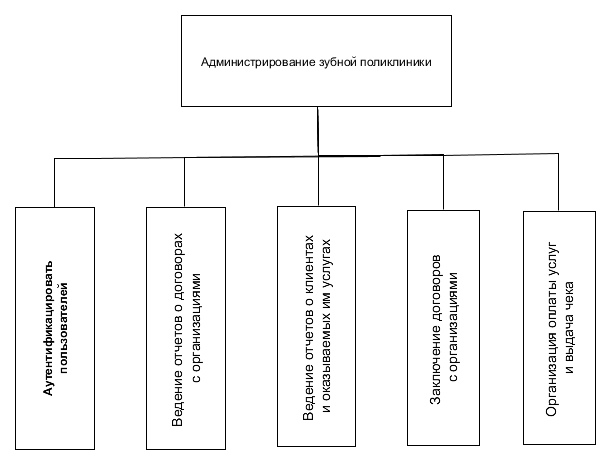
\includegraphics[width=0.7\linewidth]{images/1.jpg}\\}
		\caption{ Администрирование зубной поликлиники.}
	\end{minipage}
\end{figure}
\begin{figure}[h]
	\begin{minipage}[h]{1\linewidth}
	\centering{ 	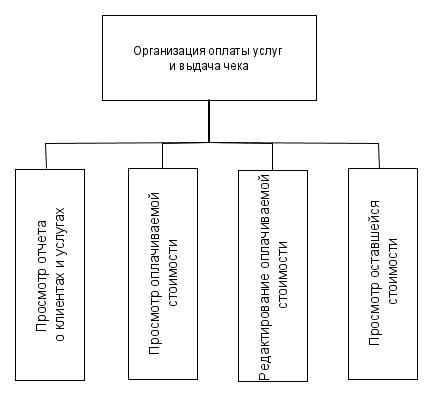
\includegraphics[width=0.53\linewidth]{images/2.jpg}\\}
	\caption{ Организация оплаты услуг и выдачи чека.}
\end{minipage}


\end{figure}

\newpage


\begin{figure}[h]
	\begin{minipage}[h]{1\linewidth}
		\centering{ 	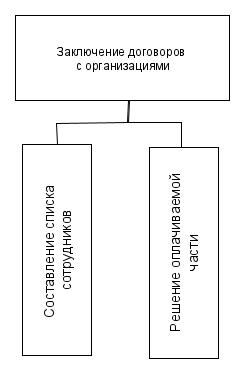
\includegraphics[width=0.4\linewidth]{images/3.jpg}\\}
		\caption{ Заключение договоров с организациями.}
	\end{minipage}
	


\end{figure}

\begin{figure}[h]

	\begin{minipage}[h]{1\linewidth}
		\centering{ 	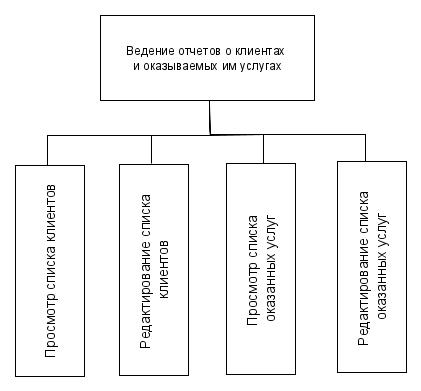
\includegraphics[width=0.44\linewidth]{images/4.jpg}\\}
		\caption{ Ведение отчетов о клиентах и оказываемых им услугах.}
	\end{minipage}
	
\end{figure}


\begin{figure}[h]
	\begin{minipage}[h]{1\linewidth}
		\centering{ 	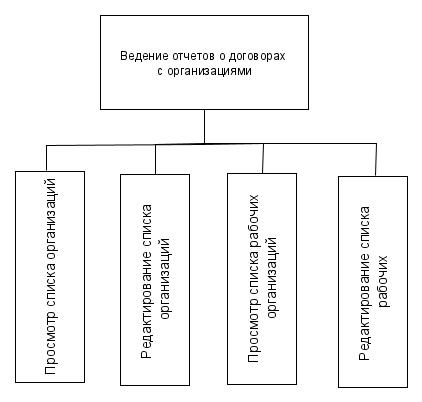
\includegraphics[width=0.6\linewidth]{images/5.jpg}\\}
		\caption{ Ведение отчетов о договорах с организациями.}
	\end{minipage}
\end{figure}



\begin{figure}[h]

	\begin{minipage}[h]{1\linewidth}
		\centering{ 	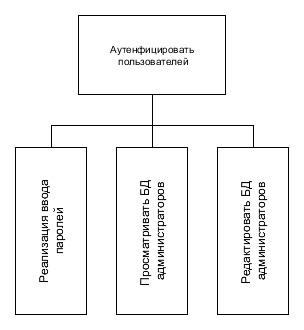
\includegraphics[width=0.5\linewidth]{images/6.jpg}\\}
		\caption{ Аутенфиция пользоватей.}
	\end{minipage}

	
\end{figure}



\clearpage
\section{ERD}

\begin{figure}[h]

	\begin{minipage}[h]{1\linewidth}
		\centering{ 	\includegraphics[width=1\linewidth]{images/ERD.jpg}\\}
		\caption{ ERD диаграмма.}
	\end{minipage}
	
\end{figure}

\clearpage
\section{Модель БД}

\begin{figure}[h]
	
	\begin{minipage}[h]{1\linewidth}
		\centering{ 	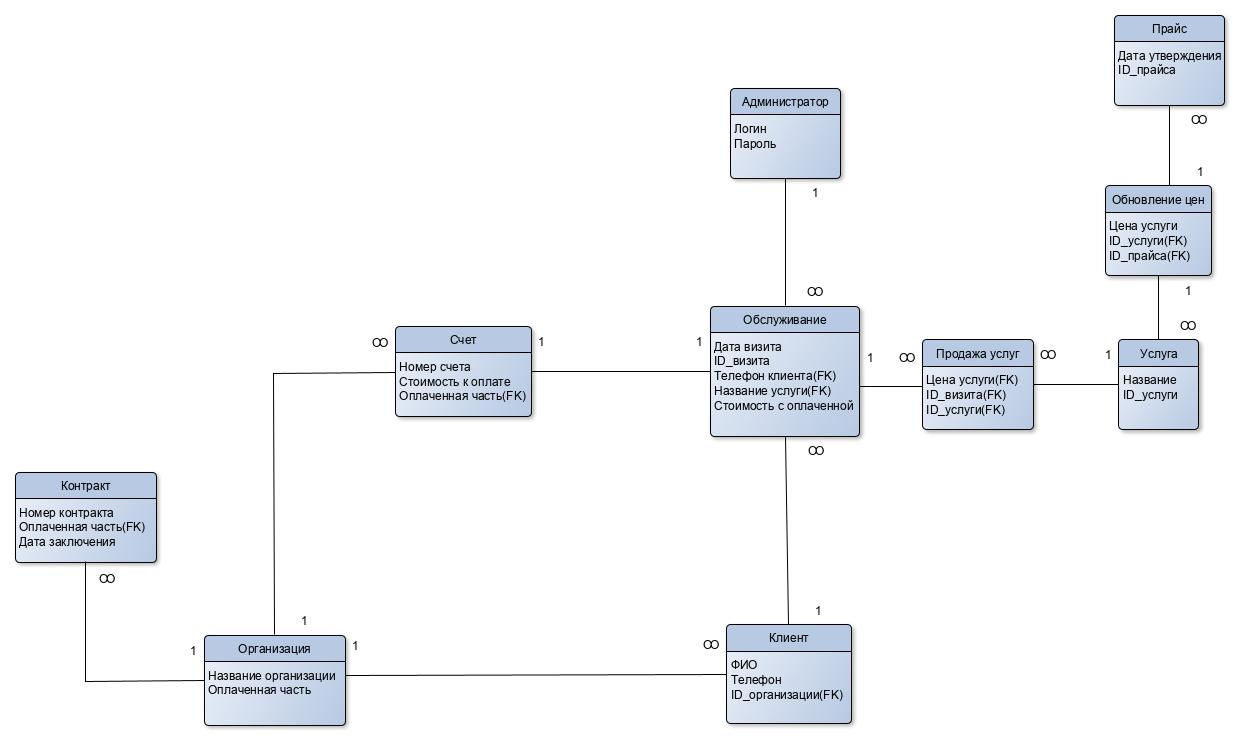
\includegraphics[width=1\linewidth]{images/REL.jpg}\\}
		\caption{Модель БД}
	\end{minipage}
	
\end{figure}









\begin{table}[h]
		\caption{Описание отношения Договор (tblContract)}
	\begin{tabular}{|l|l|l|l|}
		\hline
		\begin{tabular}[c]{@{}l@{}}Название атрибута\\ (поля)\end{tabular} & Домен (Тип данных)                                                                   & Ключи & Описание                         \\ \hline
		ContractNum                                                        & integer                                                                              & РК    & Номер контракта                  \\ \hline
		DateContract                                                       & \begin{tabular}[c]{@{}l@{}}date DEFAULT\\ CURDATE()\end{tabular}                     &       & Дата заключения контракта        \\ \hline
		ContractSum                                                        & \begin{tabular}[c]{@{}l@{}}numeric(7,2) \\ CHECK (VALUE \textgreater 0)\end{tabular} &       & Контрактные средства на человека \\ \hline
				CompanyId                                                        & integer                                                                              & FК(tblCompany)    &    Идентификатор компании           \\ \hline
	\end{tabular}
\end{table}






\begin{table}[h]
	\caption{Описание отношения Организация (tblCompany)}
	\begin{tabular}{|l|l|l|l|}
		\hline
		\begin{tabular}[c]{@{}l@{}}Название атрибута\\ (поля)\end{tabular} & Домен  & Ключи & Описание                  \\ \hline
		CompanyId                                                          & integer            & PK    & Идентификатор организации \\ \hline
		CompanyName                                                        & var(40) NOT NULL           &       & Название организации      \\ \hline
	\end{tabular}
\end{table}




\begin{table}[h]
		\caption{Описание отношения Клиент (tblClient)}
	\begin{tabular}{|l|l|l|l|}
		\hline
		\begin{tabular}[c]{@{}l@{}}Название атрибута\\ (поля)\end{tabular} & Домен  & Ключи          & Описание             \\ \hline
		ClientId                                                          & integer            & PK    & Идентификатор клиента \\ \hline
	
	Number                                                             & \begin{tabular}[c]{@{}l@{}}integer \\ CHECK (VALUE \textgreater 0)\end{tabular}      &    & Телефон клиента                  \\ \hline
	
	
	
		ClientName                                                         & varchar(40) NOT NULL       &                & Имя клиента          \\ \hline
		ClientLastName                                                     & varchar(35) NOT NULL       &                & Фамилия клиента      \\ \hline
		ClientMiddleName                                                   & varchar(35) NOT NULL       &                & Отчество клиента     \\
		\hline
						CompanyId                                                        & integer                                                                              & FК(tblCompany)    &    Идентификатор компании           \\ 
						\hline
			Ostatok                                                   & numeric(7,2)       &  FK(tblNewOst)              & Остаток от контрактной\\& & & суммы     \\ \hline
	\end{tabular}
\end{table}

\begin{table}[h]
	\caption{Описание отношения Администратор (tbl Admin)}
	\begin{tabular}{|l|l|l|l|}
		\hline
		\begin{tabular}[c]{@{}l@{}}Название атрибута\\ (поля)\end{tabular} & Домен  & Ключи & Описание                     \\ \hline
		AdminId                                                            & integer            & PK    & Идентификатор администратора \\ \hline
		Login                                                              & varchar(40) NOT NULL       &       & Логин                        \\ \hline
		Password                                                           & varchar(35) NOT NULL        &       & Пароль                       \\ \hline
	\end{tabular}
\end{table}










\begin{table}[h]
		\caption{Описание отношения Прайс (tblPrice)}
	\begin{tabular}{|l|l|l|l|}
		\hline
		\begin{tabular}[c]{@{}l@{}}Название атрибута\\ (поля)\end{tabular} & Домен & Ключи & Описание                 \\ \hline
		PriceId                                                            & integer            & PK    & Идентификатор обновления \\ \hline
		PriceDate                                                          & date DEFAULT CURDATE()              &       & Дата утверждения         \\ \hline
	\end{tabular}
\end{table}


\begin{table}[h]
		\caption{Описание отношения Услуга (tblService)}
	\begin{tabular}{|l|l|l|l|}
		\hline
		\begin{tabular}[c]{@{}l@{}}Название атрибута\\ (поля)\end{tabular} & Домен  & Ключи & Описание             \\ \hline
		Service                                                            & varchar(40) NOT NULL        &       & Название услуги      \\ \hline
		ServiceId                                                          & integer            & PK    & Идентификатор услуги \\ \hline
	\end{tabular}
\end{table}





\begin{table}[h]
		\caption{Описание отношения Обновление цен (tblNewPrice)}
	\begin{tabular}{|l|l|l|l|}
		\hline
		\begin{tabular}[c]{@{}l@{}}Название атрибута\\ (поля)\end{tabular} & Домен  & Ключи          & Описание                 \\ \hline
		PriceId                                                            & integer            & FK(tblPrice)   & Идентификатор обновления \\ \hline
		ServiceId                                                          & integer            & FK(tblService) & Идентификатор услуги     \\ \hline
	Price                                                              & \begin{tabular}[c]{@{}l@{}}numeric (7,2)\\ CHECK (VALUE \textgreater 0)\end{tabular} &       & Цена услуги                      \\ \hline
	\end{tabular}
\end{table}

\begin{table}[h]
			\caption{Описание отношения Продажа услуг(tblSales)}
	\begin{tabular}{|l|l|l|l|}
		\hline
		\begin{tabular}[c]{@{}l@{}}Название атрибута\\ (поля)\end{tabular} & Домен  & Ключи          & Описание             \\ \hline
		VisitId                                                            & integer            & FK(tblHandling)             & Идентификатор визита \\ \hline
		ServiceId                                                          & integer            & FK(tblService) & Идентификатор услуги \\ \hline
		Price                                                              & \begin{tabular}[c]{@{}l@{}}numeric (7,2)\\ CHECK (VALUE \textgreater 0)\end{tabular} &     FK(tblNewPrice)  & Цена услуги                      \\ \hline
	\end{tabular}
\end{table}








\begin{table}[h]
			\caption{Описание отношения Обслуживание(tblHandling)}
	\begin{tabular}{|l|l|l|l|}
		\hline
		\begin{tabular}[c]{@{}l@{}}Название атрибута\\ (поля)\end{tabular} & Домен  & Ключи          & Описание                   \\ \hline
	VisitData                                                          & \begin{tabular}[c]{@{}l@{}}date DEFAULT\\ CURDATE()\end{tabular}                     &       & Дата  визита                     \\ \hline
	
	
	VisitId                                                            & integer                                                                        & PK    & \begin{tabular}[c]{@{}l@{}}Идентификатор\\ обслуживания\end{tabular} \\ \hline
		ServiceID                                                            & integer       & FK(tblService) & Идентификатор услуги            \\ \hline
	ClientId                                                             & integer           & FK(tblClient)  & Идентификатор клиента            \\ \hline
		PricewoCom                                                         & \begin{tabular}[c]{@{}l@{}}integer\\ CHECK (VALUE \textgreater 0)  $T*$ \end{tabular}       &       & Стоимость без скидки             \\ \hline
	\end{tabular}
\centering{\\	$T*$ - триггер на изменение стоимости услуг без скидки для каждого визита при добавлении новой услуги в визит }
\end{table}
\begin{table}[h]
		\caption{Описание отношения Обновление остатков (tblNewOst)}
	\begin{tabular}{|l|l|l|l|}
		\hline
		\begin{tabular}[c]{@{}l@{}}Название атрибута\\ (поля)\end{tabular} & Домен  & Ключи          & Описание                 \\ \hline
		ClientId                                                            & integer            & FK(tblClient)   & Идентификатор клиента \\ \hline
		CheckId                                                          & integer            & FK(tblCheck) & Идентификатор чека    \\ \hline
		                                                         Ostatok    & numeric(7,2)  $T*$      &                & Остаток от контрактной суммы             \\ \hline
	\end{tabular}
\centering{\\	$T*$ - триггер на изменение текущих средств (см. Примерная структура триггера к  отношению tblCheck ).}
\end{table}

\begin{table}[h]
		\caption{Описание отношения Счет(tblCheck)
	}
	\begin{tabular}{|l|l|l|l|}
		\hline
		\begin{tabular}[c]{@{}l@{}}Название атрибута\\ (поля)\end{tabular} & Домен & Ключи & Описание           \\ \hline
		CheckId                                                            & integer            & РК    & Идентификатор чека \\ \hline
	
		
			
			
			
			
		FinalPrice                                                         & numeric(7,2)   $T*$  &       & Стоимость к оплате \\ \hline
		
		

		
	\end{tabular}
\centering{\\	$T*$ -	триггер на сравнение оставшейся суммы  по 	контракту и услуг, полученных клиентом.}
\end{table}

\clearpage
\begin{verbatim}
// T* Примерная структура триггера к  отношению tblCheck  при подсчете стоимости к
//оплате за лечение
USE InfSystem
GO
SET QUOTED_IDENTIFIER ON
GO
Create trigger Compareandchange   ON tblCheck
AFTER INSERT
AS 
DECLARE  @PersonPrice int , @Contractsum int, @Contract int  ; 
begin
select @PersonPrice=inserted.FinalPrice from inserted
select  @Contractsum = tblClient.Ostatok FROM tblClient
where tblCheck.CheckId==tblNewOst.CheckId, 
tblNewOst.ClientID==tblClient.ClientId, 
tblClient.CompanyId==tblCompany.CompanyId, 
tblCompany.CompanyId==tblContract.CompanyId
if( (@Contractsum-@PersonPrice)<=0)
Begin
UPDATE tblCheck
(SET tblCheck.FinalPrice = ABS (@Contractsum-@PersonPrice)
WHERE MAX(CheckID))and(SET tblNewOst.Ostatok= 0 where 
tblCheck.CheckId==tblNewOst.CheckId, 
tblNewOst.ClientID==tblClient.ClientId) and
 (SET tblClient.Ostatok=tblNewOst.Ostatok where 
 tblNewOst.ClientId==tblClient.ClientId)
END
else
(SET inserted.FinalPrice = 0 
WHERE MAX(CheckID)) and 
(SET tblNewOst.Ostatok=@Contractsum-@PersonPrice where 
tblCheck.CheckId==tblNewOst.CheckId, 
tblNewOst.ClientID==tblClient.ClientId) and 
(SET tblClient.Ostatok=tblNewOst.Ostatok where 
tblNewOst.ClientId==tblClient.ClientId)
END

\\T* Примерная структура  триггера на изменение стоимости услуг без скидки для
\\каждого визита при добавлении новой услуги в визит

USE InfSystem
GO
SET QUOTED_IDENTIFIER ON
GO
Create trigger NewServicesSum  ON tblHandling
AFTER INSERT
AS 
DECLARE  @ServiceSum int , @Visit int  ; 
begin
select @ServiceSum = SUM(Sales.Price) where
tblHadling.ServiceId==tblSales.ServiceId,
tblHadling.VisitId==tblSales.VisitId
SET(tblHandling.PricewoCom =  @ServieSum where 
tblHandling.VisitId==tblSales.VisitId)
END


\end{verbatim}




\end{document}